\documentclass[12pt]{article}%
\usepackage{amsfonts}
\usepackage{fancyhdr}
\usepackage{comment}
\usepackage{hyperref}
\usepackage[a4paper, top=2.5cm, bottom=2.5cm, left=2.2cm, right=2.2cm]%
{geometry}
\usepackage{times}
\usepackage{amsmath}
\usepackage{changepage}
\usepackage{amssymb}
\usepackage{graphicx}%
\setcounter{MaxMatrixCols}{30}
\newtheorem{theorem}{Theorem}
\newtheorem{corollary}[theorem]{Corollary}
\newtheorem{definition}[theorem]{Definition}
\newtheorem{lemma}[theorem]{Lemma}
\newtheorem{proposition}[theorem]{Proposition}
\newenvironment{proof}[1][Proof]{\textbf{#1.} }{\ \rule{0.5em}{0.5em}}

\begin{document}

\title{SOC 504 Reproducibility Memo} %Replace X with homework number, Y with problem number.
\author{David Liu and Sri Nimmagadda} %Write your name here
\date{\today}
\maketitle 
\section*{Background}
We are replicating the results of a paper titled \textit{Firearms and accidental deaths: Evidence from the aftermath of the Sandy Hook shooting} \cite{Levine1324}. The paper appeared in the December 2017 issue of Science and was authored by two economists from Wellesley College. We chose this paper to replicate because it is both recent and socially relevant as debates over gun control captivate the country. \\ \\
The paper's main contribution was establishing a casual link between "gun exposure" and accidental deaths. In the article, gun exposure is measured both in terms of online activity, such as google searches relating to firearms, and in terms of gun purchases. An example of an "accidental death" would be an unintentional fatal firing from a firearm. To establish the causal claim, the authors first collected health and firearm data from a variety of government entities. Then, Levine and McKnight utilized fixed effects and instrumental variables in their casual inference analysis. The paper's statistical content relating to causal treatment effect overlap heavily with this course and SOC 500. \\ \\
This memo will enumerate the specific replication objectives, recap our data collection process, and compare our results against those published in the paper. Finally, we propose extension ideas for feedback. 
\section*{Replication Targets}
It may be helpful to explicitly specify the values and quantities that we aim to replicate. All of the paper's claims are captured in its three figures and single table. The figures contain contextual data that setup the causal inference analysis, while the table is contains the regression outputs, the crux of the paper. Below, we will enumerate these four entities and their significance: 
\begin{enumerate}
	\item \textbf{Figure 1: Google Trends.} Using data from Google Trends, the authors argued that immediately after the Sandy Hook shooting, people had a greater interest in either purchasing a firearm or restoring an old one. For our replication, we will re-generate the two trend lines and compare them with the figure. \\
	\item \textbf{Figure 2: Association between exposure and death} The most important figure in the paper, the second figure establishes a correlation between exposure and accidental deaths. On the same plot, the authors overlay trends in gun purchases as well as accidental deaths. It will be important to confirm that exposure and accidental deaths both spike following Sandy Hook. \\
	\item \textbf{Figure 3: State-level trends in exposure} For visual clarity, the authors provided a geographical map highlighting states with high spikes in gun purchases following Sandy Hook. We will reproduce this state-level map.\\
	\item \textbf{Table: Causal inference analysis} This is the most important replication target. The authors perform causal inference for two subpopulations (children and adults) and for each subpopulation, use two separate methods (OLD and IV) to establish casual effect. We will verify the values of these regression coefficients.\\
\end{enumerate}
\subsection*{Restricted data}
This paper did utilize restricted data which we were not able to obtain. Nevertheless, we were able to replicate the paper's primary focus because the restricted data only supplemented the main findings. Specifically, the authors demonstrated that, at a national level, the Sandy Hook shooting was followed by greater gun exposure, which caused additional accidental deaths. They then performed the same analysis at the state level, to further back up their causal claim. However, state-level mortality data is restricted so we were not able to replicate Figure 4 and Table 1, Panel 4 from the paper.  
\section*{Data Collection}
The original paper utilized four datasets for its analysis. These datasets originated from Google Trends, the National Instant Criminal Background Check System (NICS), the National Cancer Institute's Surveillance, Epidemiology, and End Results program, and the CDC. Fortunately for us, the first three of these datasets were posted on the article's Dataverse. Then, following directions in the Dataverse README, we were able to obtain the mortality data from the CDC. The mortality data was most difficult to manage because the files were 10 GB in total. Otherwise, Dataverse enabled a relatively seamless data collection process.  
\section*{Comparison of Results}
\subsection*{Figure 1: Google Trends}
The search trends figure was the most straight forward to replicate because it only utilized one data set. The Dataverse did not contain code to replicate the figure directly, but we were able to import the data into R and generate the figure with ggplot. A side-by-side comparison of the two graphs are shown in Figures \ref{fig1:original} and \ref{fig:fig1_generated}. \\ \\
\begin{figure}[htbb]
	\begin{minipage}[b]{0.5\linewidth}
		\centering
		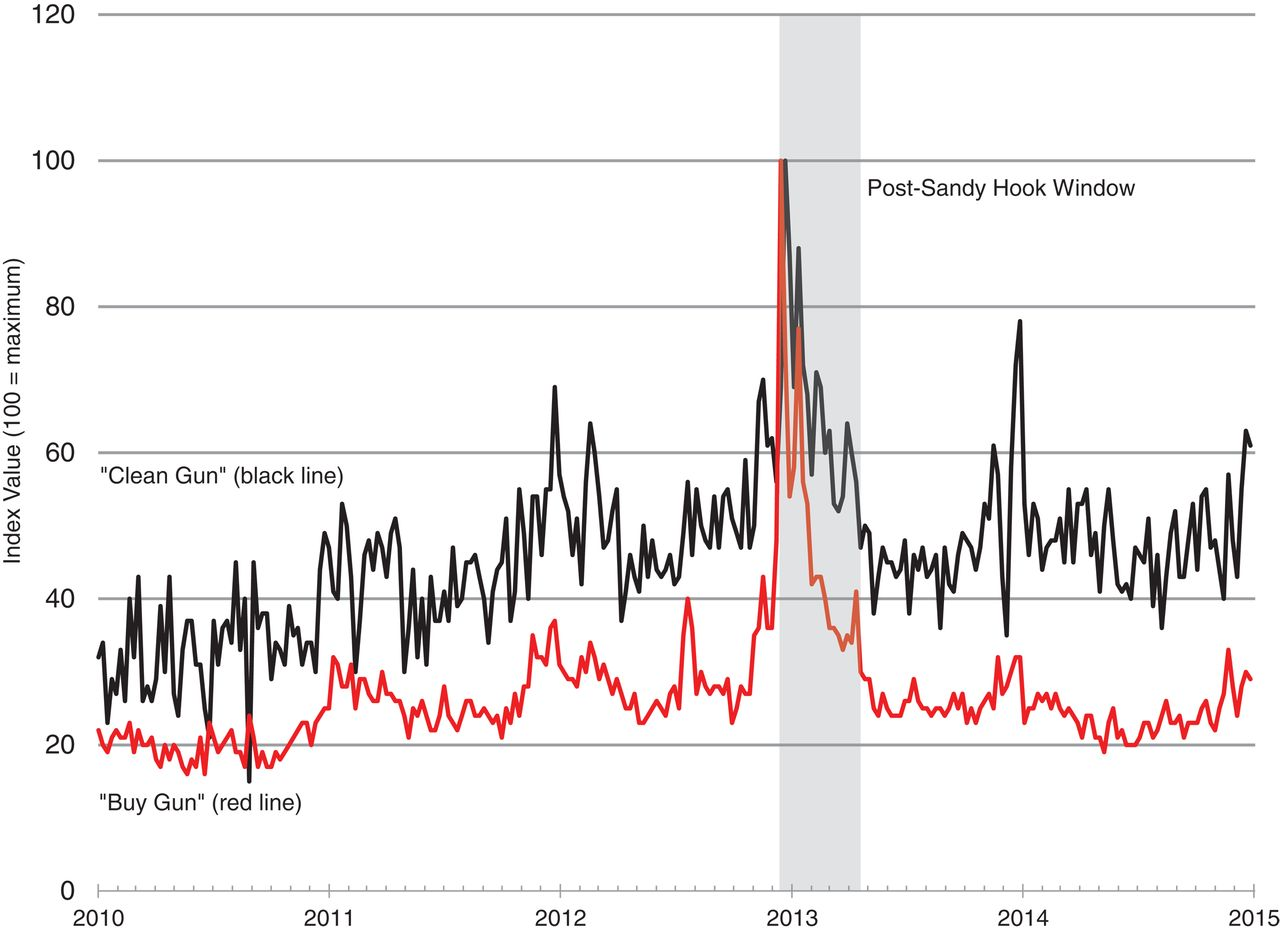
\includegraphics[width=\linewidth]{figures/fig1_original.jpg}
		\caption{Original graph}
		\label{fig:fig1_original}
	\end{minipage}
	\hspace{0.5cm}
	\begin{minipage}[b]{0.5\linewidth}
		\centering
		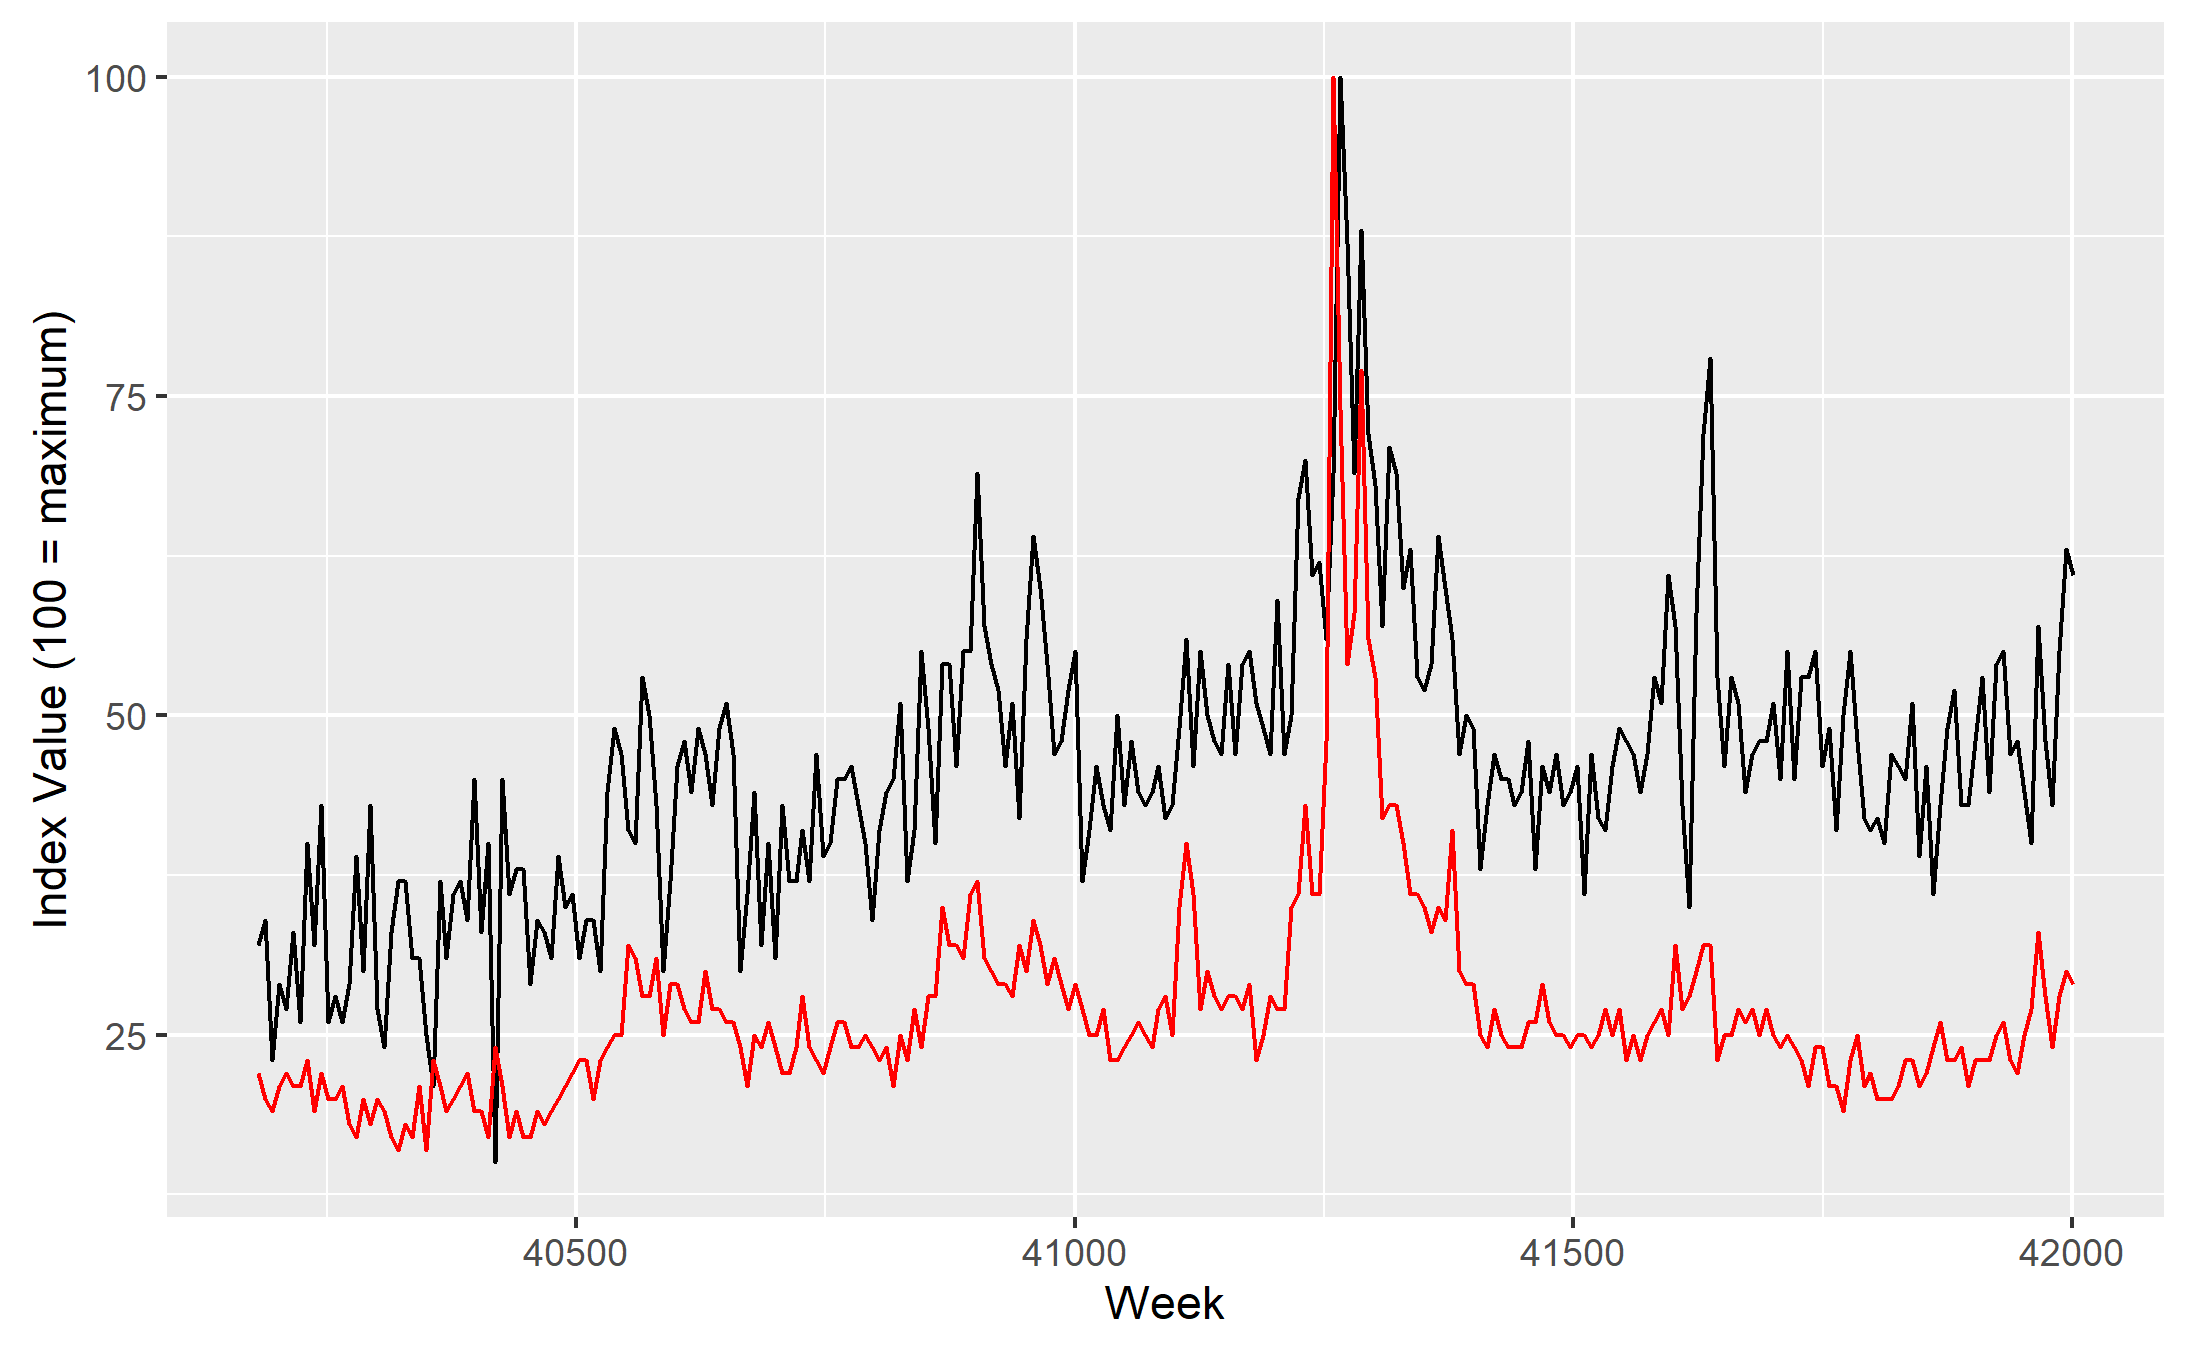
\includegraphics[width=\linewidth]{figures/fig1_generated.png}
		\caption{Generated graph}
		\label{fig:fig1_generated}
	\end{minipage}
\end{figure}
The weeks on our x-axis are still quantified in an obscure manner, the but overall trends, especially the spike following Sandy Hook, match. The original article documentation states that Google Trends data itself may be unstable depending on the time of query. We have not yet assessed this claim but plan to do so. 
\subsection*{Figure 2: Association between exposure and deaths}
This figure establishes a correlation between firearm exposure and accidental deaths, setting the stage for the causal inference that occurs later. In the replication process, we encountered a few discrepancies with the reported figures and code. We will discuss these differences in depth. \\ \\
For context, the original figure label states that the data are "deviations" from the expected values. Taking a look at the code, this wording translates into fitting regressions for firearm sales and accidental deaths, individually, and then plotting the residuals. For the firearm sales the authors fitted a fixed effects regression that accounts for monthly seasonality and yearly trends. And for the accidental deaths data, the authors fitted a quadratic function of deaths on time. There does not appear to be any documentation on why a quadratic trend was shown. \\ \\
After running the author's code, we developed the plot shown in Figures \ref{fig:fig2_sales} and \ref{fig:fig2_deaths}. For reference, the original plot is shown in Figure \ref{fig:fig2_original}. 
\begin{figure}[htbb]
	\begin{minipage}[b]{0.5\linewidth}
		\centering
		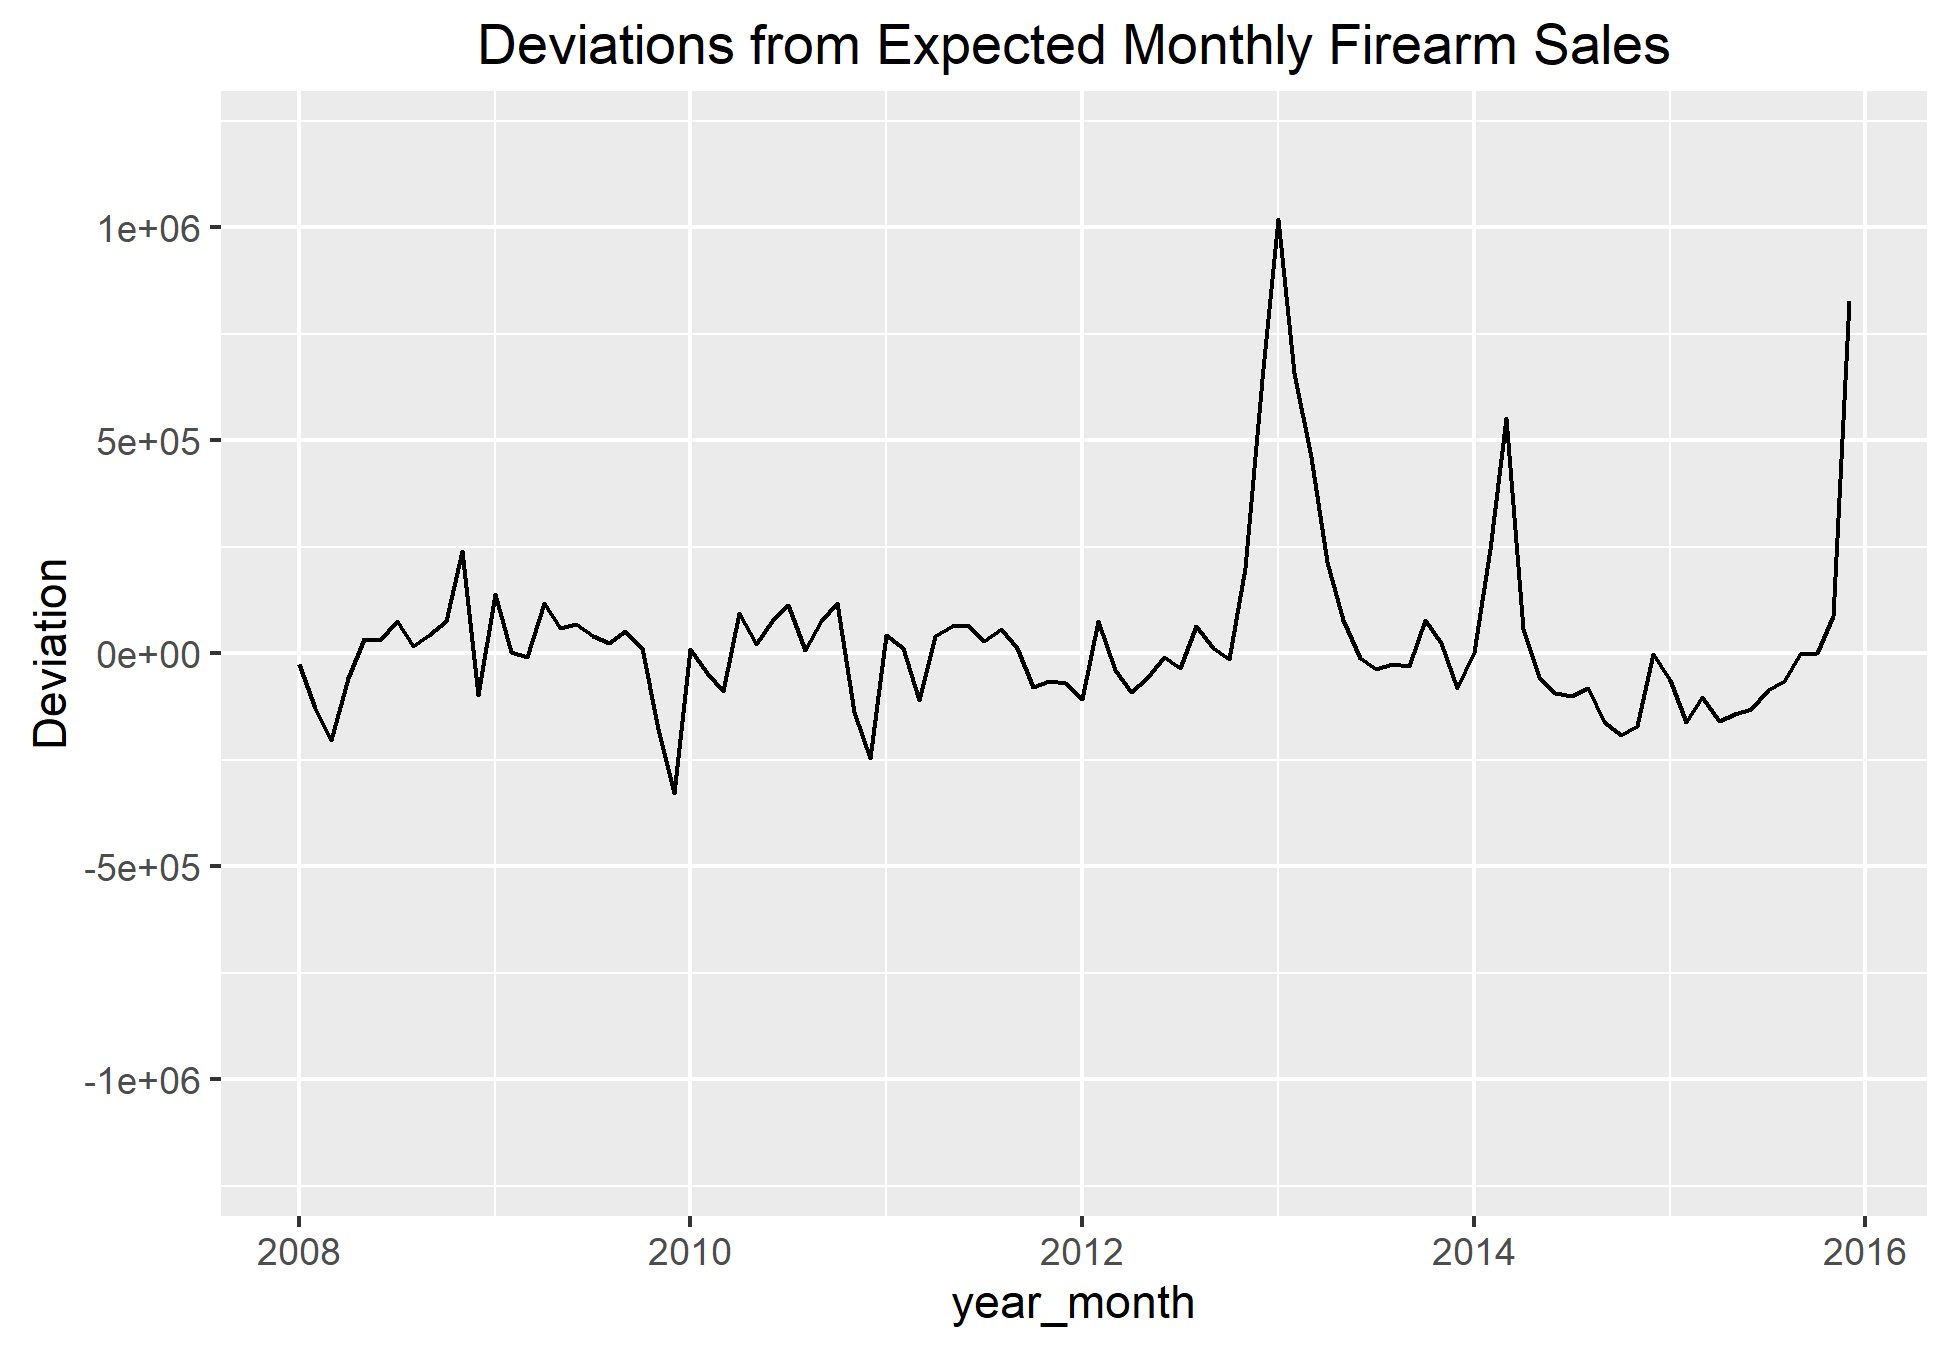
\includegraphics[width=\linewidth]{figures/fig2_sales.png}
		\caption{Sales deviations}
		\label{fig:fig2_sales}
	\end{minipage}
	\hspace{0.5cm}
	\begin{minipage}[b]{0.5\linewidth}
		\centering
		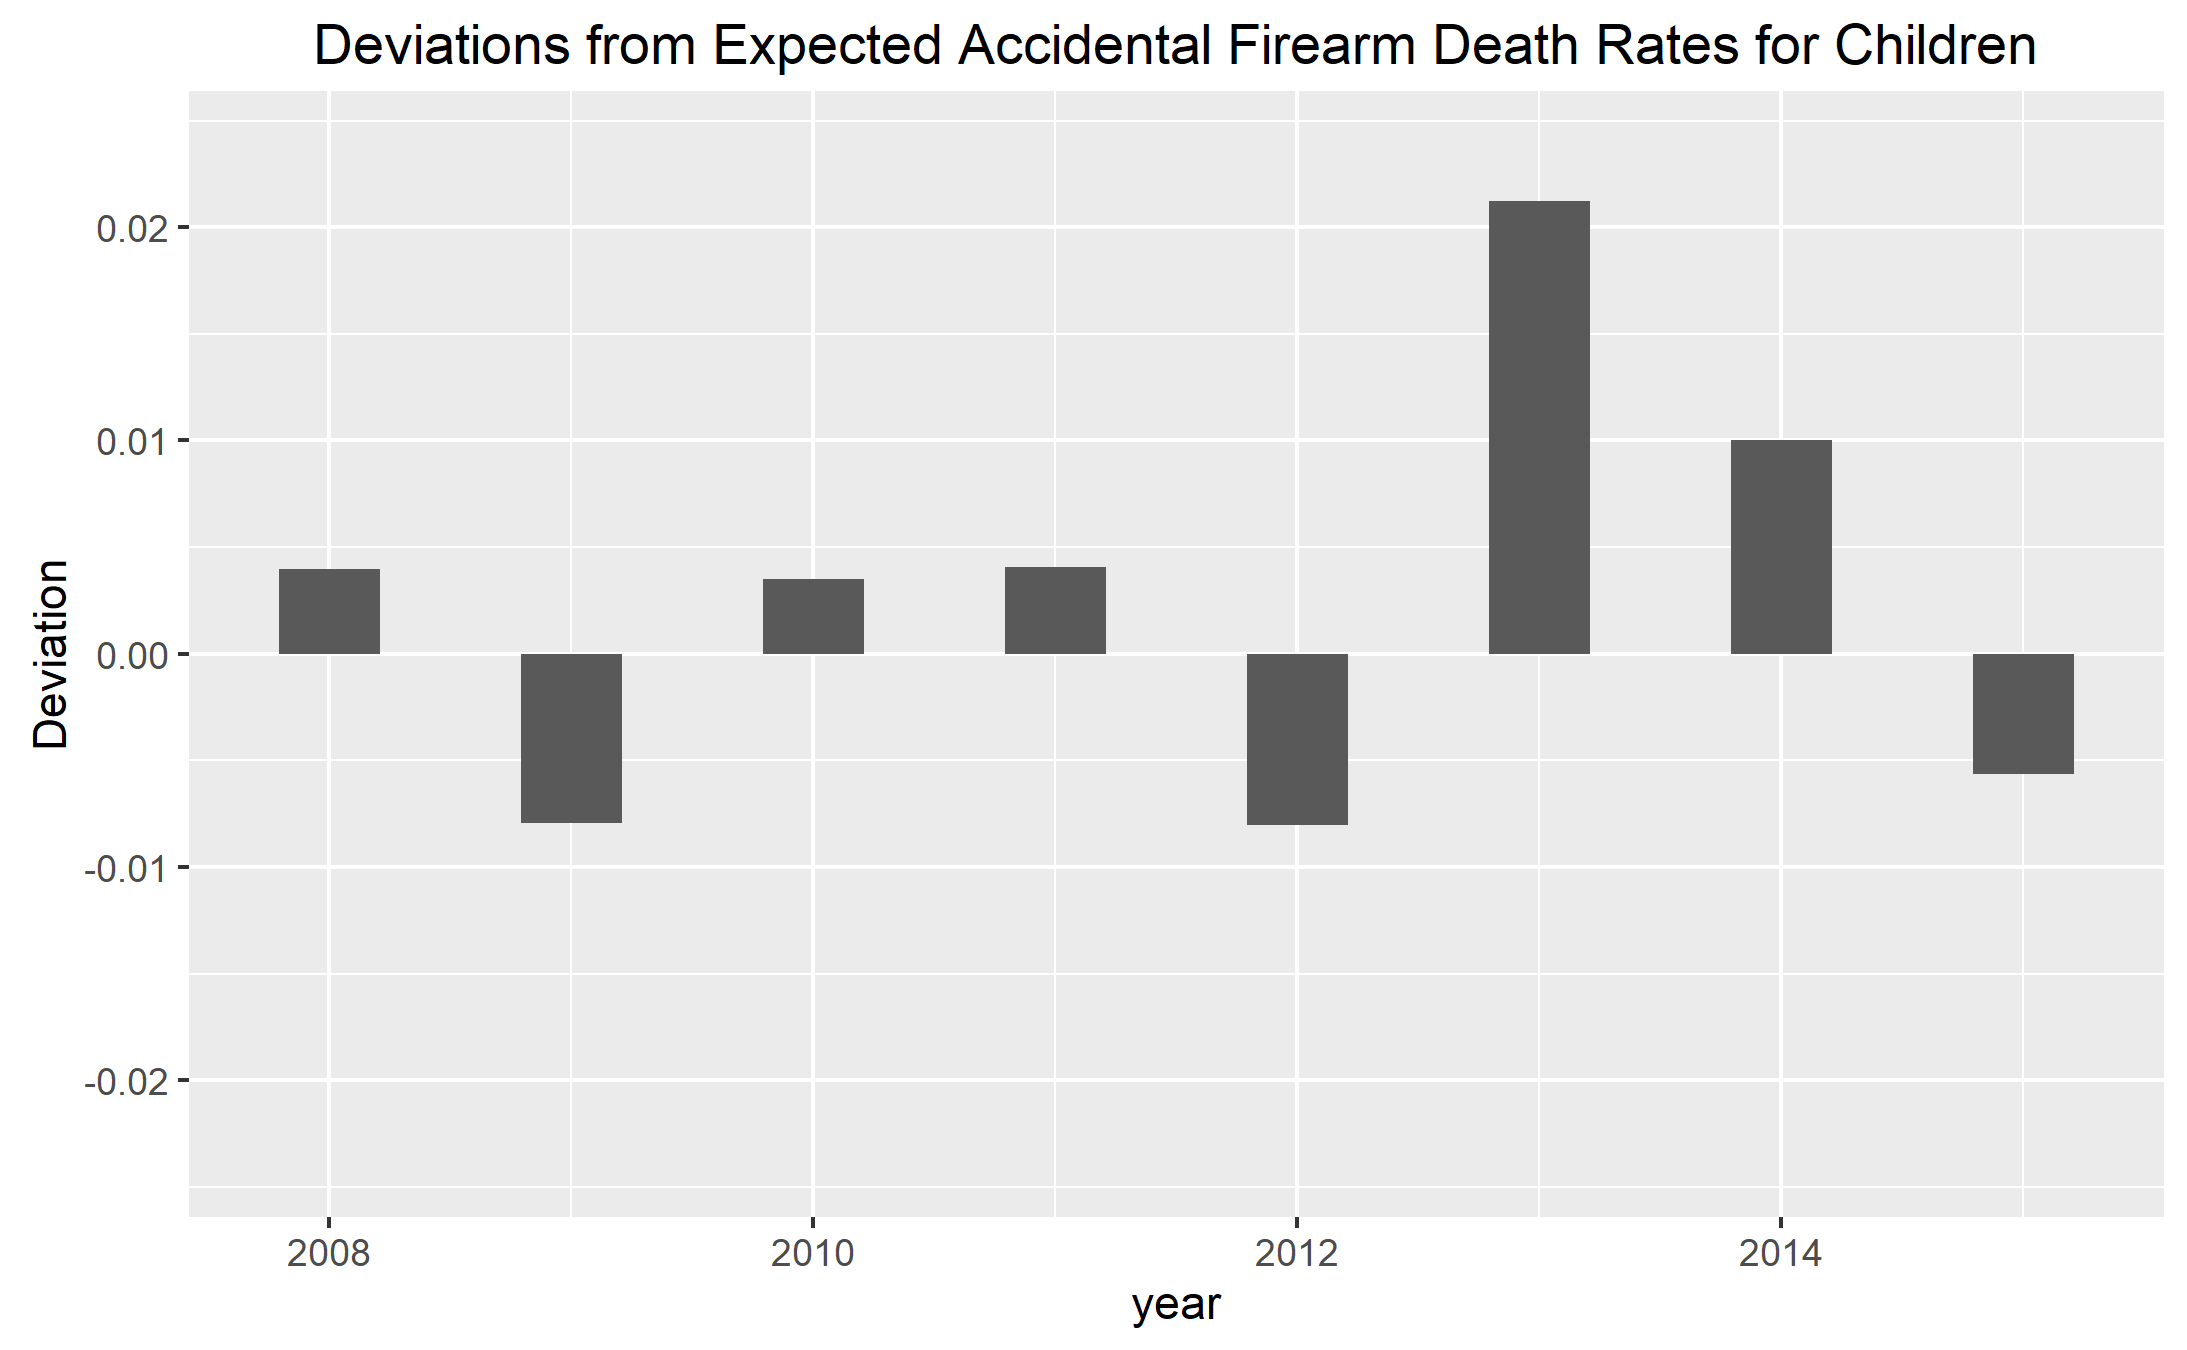
\includegraphics[width=\linewidth]{figures/fig2_deaths.png}
		\caption{Firearms deaths deviations}
		\label{fig:fig2_deaths}
	\end{minipage}
\end{figure}
\begin{figure}[hbt]
	\centering
	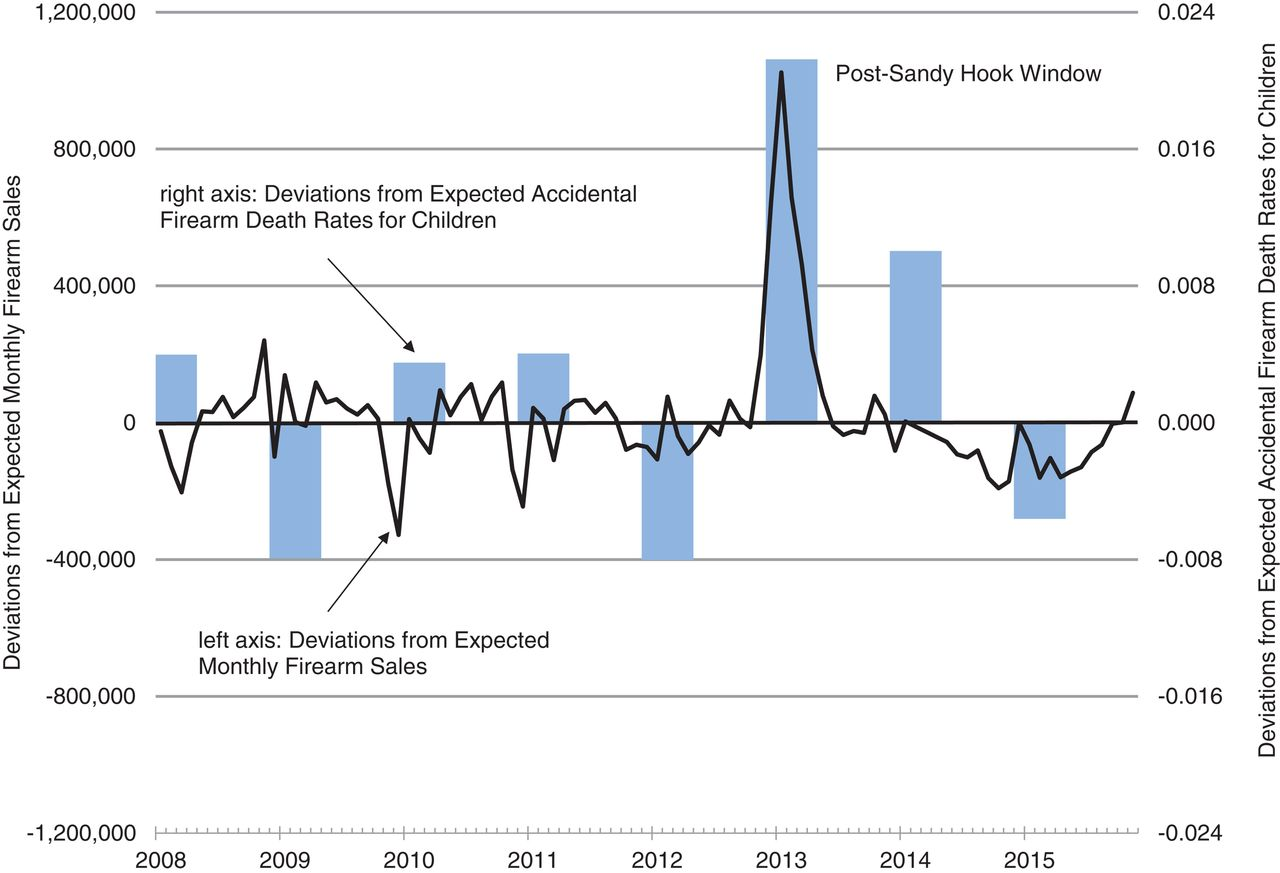
\includegraphics[width=0.75\linewidth]{figures/fig2_original.jpg}
	\caption{The original figure from the paper.}
	\label{fig:fig2_original}
\end{figure}
\subsubsection*{Discrepancies with author's results}
In order to create Figures \ref{fig:fig2_sales} and \ref{fig:fig2_deaths}, we discovered a minor bug in the author's Stata code: when building the fixed-effects regression, they mistakenly included the 2016 firearms data. In fact, when running the Stata code as-is, we generate the plot shown in Figure \ref{fig:fig2_pre_revision}. It is evident that including the 2016 data distorts the estimates for 2008 because both years must share a single fixed effects coefficient. \\ \\
\begin{figure}[hbt]
	\centering
	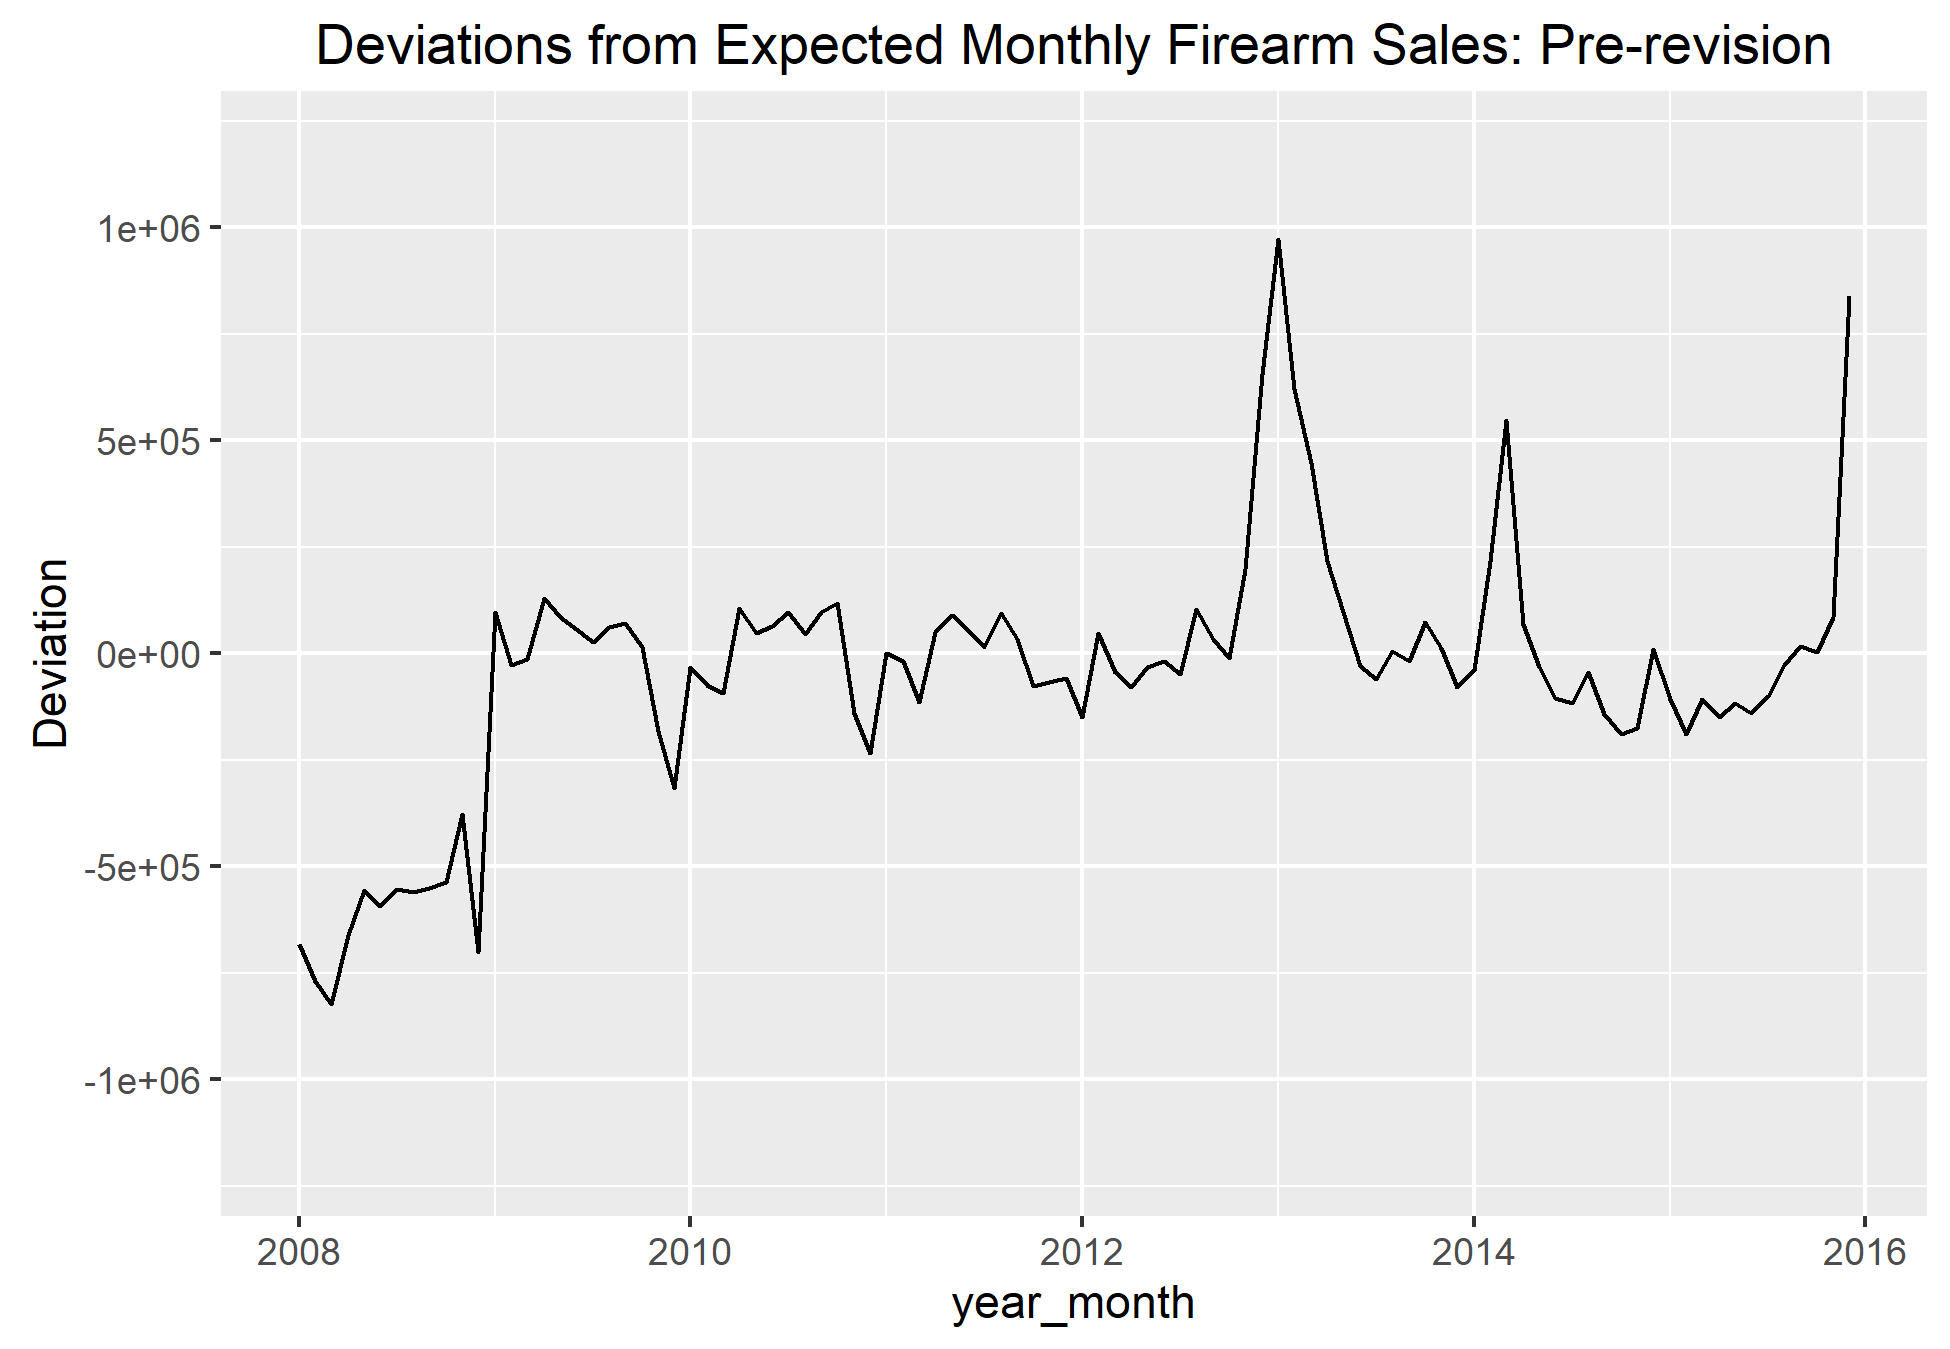
\includegraphics[width=0.75\linewidth]{figures/fig2_pre_revision.png}
	\caption{The original Stata code regressed on 2016 data which distorted estimates for 2008, the intended omitted variable.}
	\label{fig:fig2_pre_revision}
\end{figure}
Even after excluding the 2016 data, we see that the firearms deviation line plot differs from the one in the paper. Specifically, there is a noticeable peak in 2014 and the final data point, December 2015 is much higher in our plot. These values undermine the author's claim that the peak in firearm sales was unique to the Sandy-Hook area. We are still investigating the source of the discrepancy. 
\subsection*{Figure 3: State-level trends in exposure}
As a precursor to their state-level analysis, the authors demonstrated the heterogeneity in gun sale increases by state. To calculate these numbers, the authors first normalized gun purchases by state population. Then, for each state, the authors fit a fixed effects regression of gun sales on a dummy variable, which is one in the months following the shooting and zero otherwise. As before, the regression contained dummy variables to account for seasonality and annual trends. They then defined the increase in gun sales to be the coefficient on the Sandy-Hook dummy variable. \\ \\
To replicate, we simply ran the provided Stata code, which outputted a slew of regression coefficients. We then manually transferred these coefficients into a CSV data file, which maps states to gun sale increases. We then used ggplot's \texttt{geom\_map} geometry to visualize. The side-by-side comparison is shown in Figures \ref{fig:fig3_original} and \ref{fig:fig3_generated}. Though a few tweaks still need to be made, overall, these two maps match precisely. 
\begin{figure}[htbb]
	\begin{minipage}[b]{0.5\linewidth}
		\centering
		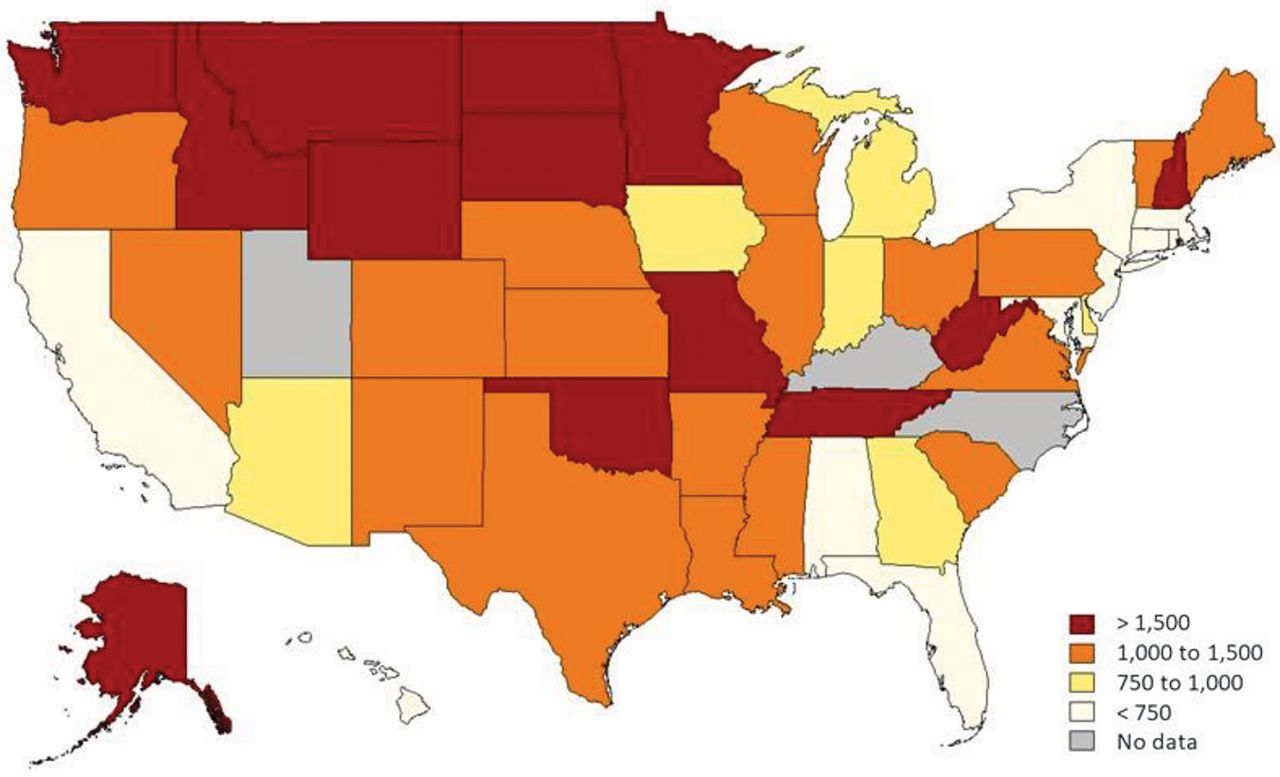
\includegraphics[width=\linewidth]{figures/fig3_original.jpg}
		\caption{Original map}
		\label{fig:fig3_original}
	\end{minipage}
	\hspace{0.2cm}
	\begin{minipage}[b]{0.5\linewidth}
		\centering
		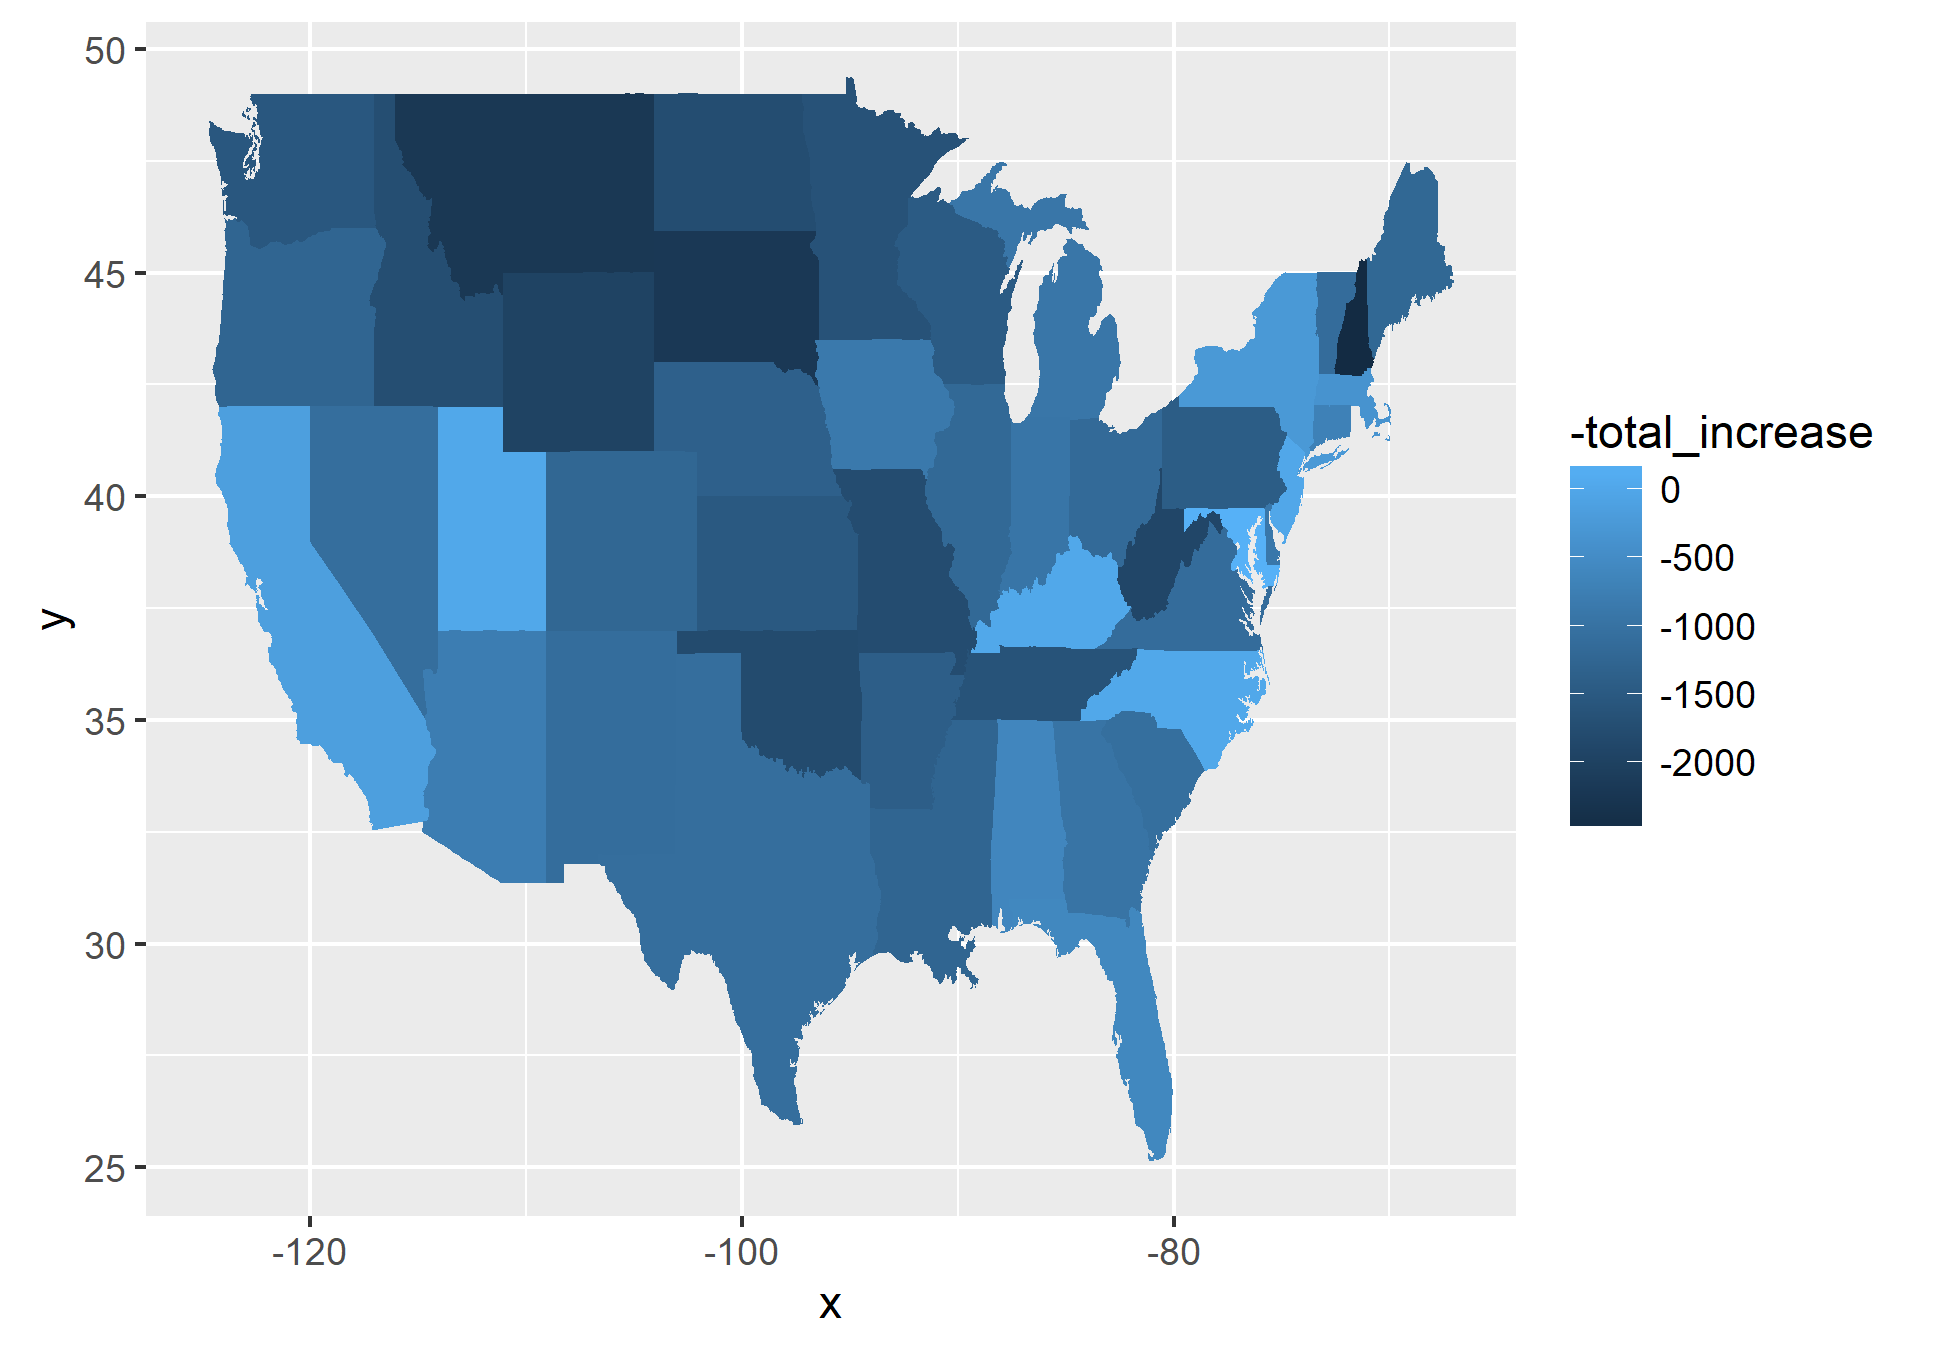
\includegraphics[width=\linewidth]{figures/fig3_generated.png}
		\caption{Generated Map}
		\label{fig:fig3_generated}
	\end{minipage}
\end{figure}
\subsection*{Causal inference analysis}
Interestingly, the paper's most significant findings were the most straight forward to replicate as many of the quantities were simply regression coefficients. To start, the original quantities are shown in Figure \ref{fig:table_original}. \\ \\
\begin{figure}[hbt]
	\centering
	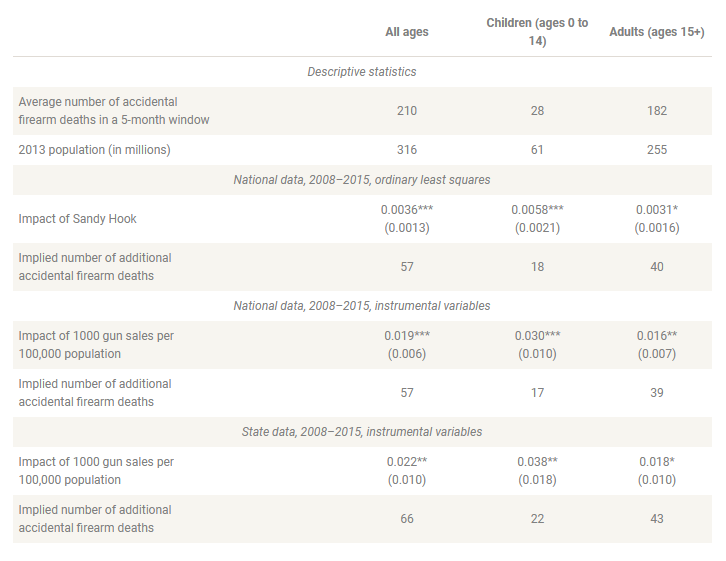
\includegraphics[width=.75\linewidth]{figures/table_original.png}
	\caption{The original reported values in Table 1, which establishes a causal relationship between firearm exposure and firearm related accidental deaths.}
	\label{fig:table_original}
\end{figure}
These first panel of the table provides descriptive statistics, such as total population and average number of accidental fire arm deaths. We ran the provided Stata code to yield the values shown in Figure \ref{fig:panel1}. The mean values of \texttt{pop byage} match the population parameters from the table. Then, if we multiply the average value of \texttt{num deaths} by five, to obtain the five-month mortality rate, we also get the average values reported in the paper.
\begin{figure}[hbt]
	\centering
	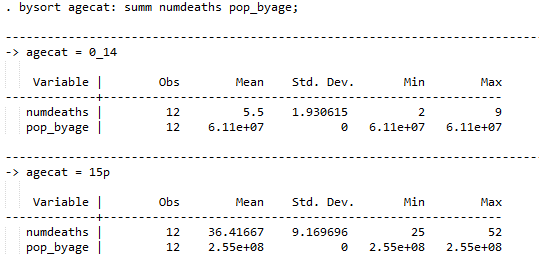
\includegraphics[width=.7\linewidth]{figures/panel1.png}
	\caption{The summary statistics from Stata concur with those from the paper.}
	\label{fig:panel1}
\end{figure}
To make causal conclusions, the authors first ran an OLS regression with a dummy variable for the Sandy Hook period representing a treatment effect. To assert that exposure produced more accidental deaths, the authors then performed an IV regression with 2 stage lease squares, where the Sandy Hook shooting was the instrument and the amount of exposure was the endogenous variable. \\ \\
In all six of these regression (two methods each applied to three age groups), we must verify the coefficient on \texttt{sandyhook}. To be concise, we do not copy those regression outputs here, but they are contained in the replication\_science.log log file. The coefficients in the final six regressions do match those reported in the paper.
\newpage 
\section*{Extension Proposals} 
We propose three separate extension ideas. Feedback will be very helpful in deciding the most promising direction to pursue. 
\subsection*{Proposal 1: Study additional mass shootings}
The most straight forward extension is to test whether the author's findings hold for other national mass shootings. The given data spans 2008 - 2016 so we have ample data to test these hypotheses. Our results would discuss the generalizeability of the original paper's findings. For example, do all mass shootings increase exposure to firearms which then leads to more accidental deaths? Looking at the overall exposure trends, our initial hypothesis is that the Sandy Hook shooting produced a truly unprecedented increase in firearm purchases. If this is the case, we can dive further into characteristics that were distinct to the Sandy Hook shooting. These results could help us address the research question: which mass shootings mobilize the public to take action? 
\subsection*{Proposal 2: Effect of gun exposure on other health outcomes}
The original paper measured the effect of gun exposure on accidental deaths, which is an arguably niche outcome variable to study. Instead, as an extension, we propose studying the effect of gun exposure on more common health outcomes. One such outcome could be mental health consequences. For instance, does being exposed to more firearms affect overall mental wellbeing. The main challenge of this approach is obtaining the necessary mental health data. Second, it would be interesting to measure the effect of gun exposure on educational performance, especially as more people have advocated for giving teachers firearms to protect students. The main hurdles to this approach would be assessing the immediacy of the firearms-exposure effect (if any on education). \\ \\ 
Nevertheless, these ideas are favorable because we already have the background checks data (firearm exposure), and we can still leverage the Sandy Hook shooting as an instrumental variable. 
\subsection*{Proposal 3: factors effecting gun purchases}
Our final proposal deviates further from the author's original objectives, but leverages their data cleaning efforts and potentially carries greater political weight. Instead of treating the number of firearm background checks as an independent variable, we are interested in using it as an outcomes variable. Presently, thanks to the original author's meticulous data cleaning, we have data on the number of background checks that occurred in each state in each month between 2008 - 2016. It would be interesting to measure the effect of various control laws on the actual number of firearms purchased. These laws could help us quantify the decrease in firearm background checks following gun control legislation. Alternatively, we could measure the potentially positive effect of media advertising (such as those from the NRA) on background checks. For this proposal, we would collect data from social media, such as Twitter, and measure the network effects driving firearm sales.  
\bibliographystyle{IEEEtranS}
\bibliography{references}
\section*{Appendix}
\subsection*{\href{https://dataverse.harvard.edu/dataset.xhtml?persistentId=doi:10.7910/DVN/EVLKBN}{Dataverse}} 
The original Dataverse (hosted by Harvard) contains the raw background checks, population, and trends data. It also contains the two Stata files used for data cleaning and analysis. 
\subsection*{\href{https://github.com/dliu18/firearms-replication}{Project Github}}
We have posted all of the code and data used for replication in the private Github repository above. 
\subsection*{Supplemental Materials}
In the Google Drive folder, we have included a supplemental materials document. This file contains the Stata log-file from running the provided code as well as the R markdown document we wrote to generate the figures. 
\end{document}